\chapter{ITERATOR}

Pattern \underline{comportamentale}, descrivono come classi e oggetti interagiscono e si distribuiscono le responsabilità.

Usato per accedere ai contenuti di un oggetto aggregato senza esporne la rappresentazione interna e fornisce un modo uniforme per attraversarla.
\smallskip

Supponiamo di avere una classe scuola, avente una collezione privata di studenti permettendo ai client di poter aggiungere alla collezione col metodo add() e di 
volerne dare un accesso in sola lettura, attraverso un getter pubblico
\begin{lstlisting}
public class School {
    private ArrayList<Student> students = new ArrayList<>();
    
    public void addStudent(Student student) {
        students.add(student);
    }
    
    public ArrayList<Student> getStudents() {
        return students;
    }
}
\end{lstlisting}

Così facendo si espone ai client un dettaglio implementativo, ArrayList e, se un giorno decidessi di cambiare l'implementazione della collezione, i client avranno 
problemi di compilazione.

Un getter protected non migliorerebbe la situazione in quanto ai client esterni basterebbe estendere la nostra classe per usare quel getter e quindi stesso problema.
\smallskip

Utilizzando un iteratore
\begin{itemize}
    \item accediamo ai contenuti di oggetto aggregato senza esporne la rappresentazione interna;
    \item possiamo supportare diverse strategie di attraversamento;
    \item fornire un’interfaccia uniforme per attraversare strutture aggregate diverse.
\end{itemize}

\textbf{N.B.} Un iteratore non conosce il numero di elementi di un aggregato, può solamente attraversarli.
\medskip

Quindi con l'iteratore avremo
\begin{lstlisting}
public class School {
    private List<Student> students = new ArrayList<>();
    
    public void addStudent(Student student) {
        students.add(student);
    }

    public Iterator<Student> studentIterator() {
        return students.iterator();
    }
}
\end{lstlisting}

dove i client usano studentIterator() per “attraversare” sequenzialmente i vari studenti della scuola, ignorando completamente la rappresentazione interna della 
struttura che li contiene senza poter fare assunzioni sull’ordine durante l’attraversamento.

\medskip
\textbf{N.B.} Una volta usato un iteratore per un attraversamento completo, ne va usato uno nuovo.

\section{Struttura}

\begin{figure}[H]
    \centering
    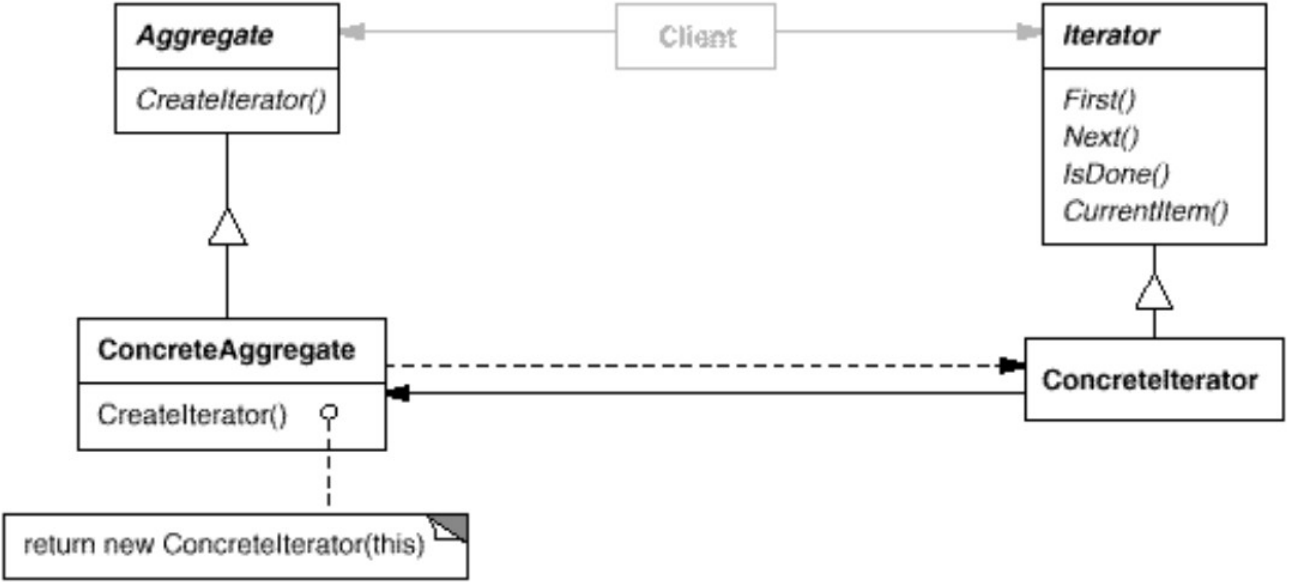
\includegraphics[width=0.5\linewidth]{../../immagini/iterator/struttura_visitor}
\end{figure}

\textbf{Iterator} definisce l'interfaccia per attraversare gli elementi e offre metodi come hasNext() per verificare se ci sono altri elementi da attraversare e next()
per ottenere l'elemento successivo;

\textbf{Aggregate} è l'interfaccia, o la classe astratta, che rappresenta la collezione di oggetti che fornisce un metodo per ottenere un iteratore che può essere 
utilizzato per attraversare gli elementi;

\textbf{ConcreteIterator} implementa Iterator, tiene traccia, durante l’attraversamento, dell’oggetto corrente, deve essere in grado di calcolare l’elemento 
successivo e ha un riferimento all’aggregato concreto;

\textbf{ConcreteAggregate} implementa Aggregate e crea un opportuno ConcreteIterator.

\section{Iterator e classi anonime}

Un iteratore concreto è tipicamente implementato come classe (privata) interna o direttamente come classe anonima, infatti deve poter accedere direttamente alla
rappresentazione interna (privata) dell’aggregato.
\begin{lstlisting}
public class School {
    private Student[] students = new Student[100];
    private int index = 0;
    
    public void addStudent(Student student) {
        // controlli per la dimensione da fare...
        students[index++] = student;
    }

    public Iterator<Student> studentIterator() {
        return new Iterator<Student>() {
            private int current = 0;

            @Override
            public boolean hasNext() {
                return current < index;
            }

            @Override
            public Student next() {
                if (current >= index)
                    throw new NoSuchElementException();
                return students[current++];
            }
        };
    }
}
\end{lstlisting}

\section{Iterator vs Stream}

Possono sembrare simili ma
\begin{itemize}
    \item gli stream sono più astratti e possono essere parallelizzati, si basano su un approccio dichiarativo, permettono facilmente di filtrare, raggruppare, 
    partizionare e \underline{gestiscono, in automatico, l’attraversamento dell’aggregato};
    \item gli iteratori sono molto più semplici, permettono di attraversare un aggregato un elemento alla volta, sono per loro stessa natura sequenziali ma 
    richiedono \underline{che hasNext() e next() siano usati correttamente insieme};
    \item creare un’implementazione di Iterator è piuttosto semplici, i metodi da implementare sono pochi;
    \item creare un’implementazione di Stream non è banale.
\end{itemize}